% !TeX program = xelatex
\documentclass[a4paper,10pt]{article}

% ============================================================================
% សន្លឹកកិច្ចការសិស្ស ស-ខ្មៅ (Student Fill-In Worksheet — No-LCD Classroom)
% មេរៀនទី១៧ (១៧.១.៣)៖ ផ្ទៃក្រឡាខាងនិងផ្ទៃក្រឡាទាំងអស់នៃកោន (ត្រូវគ្នា ១០០% នឹង LS_Plan_CONE_SA.tex)
% ============================================================================
\usepackage[a4paper, left=0.95cm, right=0.95cm, top=0.75cm, bottom=0.90cm, footskip=0.48cm]{geometry}
\usepackage{amsmath}
\usepackage{unicode-math}
\usepackage{fontspec}
\usepackage{array, colortbl}
\usepackage[table]{xcolor}
\usepackage{enumitem}
\usepackage{pifont}
\usepackage{fancyhdr}
\usepackage{lastpage}
\usepackage{tikz}
\usepackage[most]{tcolorbox}
\usetikzlibrary{calc, arrows.meta, angles, quotes, patterns, decorations.markings, babel}

\makeatletter
\let\@expl@@@mark@update@singlecol@structures@@\relax
\makeatother

\providecommand{\NGSFindFonts}{%
  \IfFileExists{C:/Windows/Fonts/cambria.ttc}{%
    \def\NGSSysPath{C:/Windows/Fonts/}%
    \def\NGSUserPath{C:/Users/KIT/AppData/Local/Microsoft/Windows/Fonts/}%
  }{%
    \IfFileExists{./fonts/KhmerOSsiemreap.ttf}{\def\NGSSysPath{./fonts/}\def\NGSUserPath{./fonts/}}{%
    \IfFileExists{../fonts/KhmerOSsiemreap.ttf}{\def\NGSSysPath{../fonts/}\def\NGSUserPath{../fonts/}}{%
    \IfFileExists{../../fonts/KhmerOSsiemreap.ttf}{\def\NGSSysPath{../../fonts/}\def\NGSUserPath{../../fonts/}}{%
    \IfFileExists{../../../fonts/KhmerOSsiemreap.ttf}{\def\NGSSysPath{../../../fonts/}\def\NGSUserPath{../../../fonts/}}{%
    \IfFileExists{../../../../fonts/KhmerOSsiemreap.ttf}{\def\NGSSysPath{../../../../fonts/}\def\NGSUserPath{../../../../fonts/}}{%
    \IfFileExists{../../../../../fonts/KhmerOSsiemreap.ttf}{\def\NGSSysPath{../../../../../fonts/}\def\NGSUserPath{../../../../../fonts/}}{%
    \IfFileExists{../../../../../../fonts/KhmerOSsiemreap.ttf}{\def\NGSSysPath{../../../../../../fonts/}\def\NGSUserPath{../../../../../../fonts/}}{%
      \def\NGSSysPath{../../../../../../../fonts/}\def\NGSUserPath{../../../../../../../fonts/}%
    }}}}}}}%
  }%
}
\NGSFindFonts

\setmathfont[Path={\NGSSysPath}, FontIndex=1, Scale=1.02]{cambria.ttc}
\defaultfontfeatures{Ligatures=TeX}

\setmainfont[
  Path={\NGSUserPath},
  Extension=.ttf,
  Script=Khmer,
  BoldFont={KhmerOSsiemreap},
  BoldFeatures={FakeBold=1.8},
  ItalicFont={KhmerOSsiemreap},
  ItalicFeatures={FakeSlant=0.25},
  BoldItalicFont={KhmerOSsiemreap},
  BoldItalicFeatures={FakeBold=1.8, FakeSlant=0.25}
]{KhmerOSsiemreap}

\newfontfamily\muol[Path={\NGSUserPath}, Extension=.ttf, Script=Khmer]{KhmerOSmuollight}
\newfontfamily\TimesEn[Path={\NGSSysPath}, Extension=.ttf, BoldFont={timesbd}, ItalicFont={timesi}, BoldItalicFont={timesbi}]{times}

\XeTeXlinebreaklocale "km"
\XeTeXlinebreakskip = 0pt plus 1pt minus 0.1pt

\definecolor{panelgray}{gray}{0.93}
\definecolor{headgray}{gray}{0.85}

\pagestyle{fancy}
\fancyhf{}
\renewcommand{\headrulewidth}{0pt}
\fancyfoot[L]{\fontsize{8pt}{10pt}\selectfont អនុវិទ្យាល័យព្រះក្រសាំង \en{---} គណិតវិទ្យា ថ្នាក់ទី៨ \en{|} មេរៀនទី១៧ (១៧.១ ផ្ទៃក្រឡាខាងនិងផ្ទៃក្រឡាទាំងអស់នៃកោន)}
\fancyfoot[R]{\fontsize{8.2pt}{10pt}\selectfont ទំព័រ \en{\thepage\ / \pageref{LastPage}}}

\setlength{\parindent}{0pt}
\setlength{\parskip}{0pt}
\setlength{\tabcolsep}{4pt}

\newcommand{\en}[1]{{\TimesEn #1}}
\newcommand{\enbf}[1]{{\TimesEn\textbf{#1}}}
\newcommand{\unit}[1]{\,\text{\en{#1}}}
\newcommand{\cnum}[1]{\mbox{\fontsize{10pt}{12pt}\selectfont\ding{\numexpr181+#1\relax}}}
\newcommand{\chkbox}{\tikz[baseline=-0.15ex]\draw[black, line width=0.85pt] (0,0) rectangle (0.25cm,0.25cm);}
\newcommand{\blank}[1]{\makebox[#1]{\dotfill}}

\newcommand{\rightbox}[4][0.18]{%
  \draw[black, line width=0.8pt]
    ($(#3)!#1!(#2)$) -- ($($(#3)!#1!(#2)$)+($(#3)!#1!(#4)$)-(#3)$) -- ($(#3)!#1!(#4)$);
}

\newcommand{\secbar}[2]{%
  \vspace{3pt}%
  \begin{tcolorbox}[
    enhanced, sharp corners, colback=headgray, colframe=black,
    boxrule=0.9pt, boxsep=1pt, top=2.5pt, bottom=2.5pt, left=6pt, right=6pt,
    after skip=3pt
  ]
    {\muol\fontsize{9.2pt}{13.5pt}\selectfont #1}\hfill{\fontsize{8.3pt}{11.5pt}\selectfont\textbf{#2}}
  \end{tcolorbox}%
}

\newcolumntype{L}[1]{>{\raggedright\arraybackslash}p{#1}}
\newcolumntype{C}[1]{>{\centering\arraybackslash}p{#1}}

\begin{document}
\fontsize{9.4pt}{13.8pt}\selectfont

% ============================================================================
% ទំព័រទី ១៖ ក្បាលសន្លឹកកិច្ចការ + E1 + E2 (ពន្លាតចម្រៀកថាស & គំរូទី 1, 2) + E3 (រូបមន្ត & អន្ទាក់ទិន្នន័យ)
% ============================================================================
\begin{tcolorbox}[
  enhanced, sharp corners, colback=white, colframe=black,
  boxrule=1.1pt, boxsep=2.5pt, top=5.5pt, bottom=5.5pt, left=6pt, right=6pt, after skip=6.5pt
]
  \begin{center}
    {\muol\fontsize{10pt}{14.5pt}\selectfont សន្លឹកកិច្ចការសិស្ស \enbf{---} គណិតវិទ្យា ថ្នាក់ទី៨ \enbf{(}១៧\enbf{.}១ ផ្ទៃក្រឡាខាងនិងផ្ទៃក្រឡាទាំងអស់នៃកោន\enbf{)}}\\[3.5pt]
    {\fontsize{8.8pt}{12pt}\selectfont
    ឈ្មោះសិស្ស / ដៃគូ៖ \blank{6.2cm} \hspace{0.2cm}
    ថ្នាក់៖ \blank{1.4cm} \hspace{0.2cm}
    ក្រុម៖ \blank{1.2cm} \hspace{0.2cm}
    កាលបរិច្ឆេទ៖ \blank{2.8cm}}
  \end{center}
\end{tcolorbox}

% --- E1 Engage ---
\begin{tcolorbox}[
  enhanced, sharp corners, colback=panelgray, colframe=black,
  boxrule=0.8pt, boxsep=2.5pt, top=5.5pt, bottom=5.5pt, left=6pt, right=6pt, after skip=6.5pt
]
  \textbf{បេសកកម្មទី១ (\en{E1 - Engage})៖ មួកក្រដាសរាងកោនបរិវត្ត — ពេលកាត់ពន្លាតតាមជនេត្រមួយ បានរូបអ្វី?}\\[2.5pt]
  សិស្សម្នាក់ធ្វើមួកក្រដាសរាងកោនបរិវត្តមានកាំបាត $r=2\unit{cm}$ និងជនេត្រ $s=6\unit{cm}$ ។ ពេលកាត់ពន្លាតផ្ទៃខាងតាមជនេត្រ $s$៖ \textbf{មិត្ត ក} ថាបានរូបត្រីកោណមានបាត $4\unit{cm}$ ឯ \textbf{មិត្ត ខ} ថាបានរូប \textbf{ចម្រៀកថាស} ដែលមានកាំស្មើជនេត្រ $s$ និងប្រវែងធ្នូស្មើបរិមាត្របាត $2\pi r$!\\[2.5pt]
  \ding{226}\ ចូរទស្សន៍ទាយជាដៃគូ៖ \;\chkbox\ មិត្ត ក ត្រឹមត្រូវ \hspace{0.5cm} \chkbox\ មិត្ត ខ ត្រឹមត្រូវ \hspace{0.5cm} \chkbox\ ទាំងពីរស្មើគ្នា
\end{tcolorbox}

% --- E2 Explore Part A: Sector-to-Parallelogram Slicing ---
\secbar{ផ្នែកទី១ \enbf{(}ក\enbf{)} ៖ ពន្លាតផ្ទៃខាងកោនជាចម្រៀកថាស និងផ្គុំប្រលេឡូក្រាម \enbf{(E2 - Explore)}}{ការងារជាដៃគូ \en{5 min}}

\noindent
\begin{minipage}[c]{9.3cm}
  \centering
  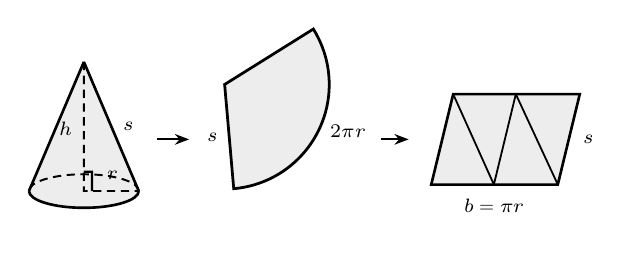
\begin{tikzpicture}[scale=0.82, every node/.style={font=\scriptsize, text=black}]
    % (1) កោន 3D
    \begin{scope}[shift={(-3.55,0)}]
      \coordinate (V) at (0,1.35);
      \coordinate (O) at (0,-0.65);
      \coordinate (L) at (-0.85,-0.65);
      \coordinate (R) at (0.85,-0.65);
      \fill[gray!14] (L) -- (V) -- (R) arc (0:-180:0.85 and 0.26);
      \draw[black, line width=0.95pt] (L) arc (-180:0:0.85 and 0.26) (V) -- (L) (V) -- (R);
      \draw[black, line width=0.7pt, densely dashed] (R) arc (0:180:0.85 and 0.26) (V) -- (O) -- (R);
      \rightbox[0.15]{V}{O}{R}
      \node[above=0.5pt] at (0.45,-0.65) {$r$};
      \node[left=0.5pt] at (0,0.32) {$h$};
      \node[right=1pt] at ($0.5*(V)+0.5*(R)$) {$s$};
      \node at (0,-1.35) {\textbf{កោនបរិវត្ត}};
    \end{scope}

    \draw[-{Stealth[length=1.8mm]}, line width=0.8pt] (-2.42,0.15) -- (-1.92,0.15);

    % (2) ចម្រៀកថាស
    \begin{scope}[shift={(-0.72,0.20)}]
      \coordinate (C) at (-0.65,0.80);
      \fill[gray!14] (C) -- ($(C)+(-85:1.62)$) arc (-85:32:1.62) -- cycle;
      \draw[black, line width=1.0pt] (C) -- ($(C)+(-85:1.62)$) arc (-85:32:1.62) -- cycle;
      \node[left=0.5pt] at ($(C)+(-85:0.82)$) {$s$};
      \node[right=0.5pt] at ($(C)+(-26:1.64)$) {$2\pi r$};
      \node at (-0.05,-1.55) {\textbf{ចម្រៀកថាស}};
    \end{scope}

    \draw[-{Stealth[length=1.8mm]}, line width=0.8pt] (1.05,0.15) -- (1.48,0.15);

    % (3) ប្រលេឡូក្រាម
    \begin{scope}[shift={(3.05,0.10)}]
      \draw[black, line width=0.95pt, fill=gray!14] (-1.22,-0.65) -- (-0.88,0.75) -- (1.08,0.75) -- (0.74,-0.65) -- cycle;
      \draw[black, line width=0.65pt] (-0.25,-0.65) -- (0.09,0.75) (-0.88,0.75) -- (-0.25,-0.65) (0.09,0.75) -- (0.74,-0.65);
      \node[below=1pt] at (-0.25,-0.68) {$b = \pi r$};
      \node[right=1pt] at (0.94,0.05) {$s$};
      \node at (-0.10,-1.45) {\textbf{ប្រលេឡូក្រាម}};
    \end{scope}
  \end{tikzpicture}
\end{minipage}%
\hfill
\begin{minipage}[c]{9.3cm}\raggedright
  \textbf{បំពេញតាមសៀវភៅទំព័រ ២២០--២២១៖}\\[6pt]
  $1.$ កោនបរិវត្តមានបាតជា \textbf{\blank{1.6cm}} កាំ $r$ (ផ្ទៃបាត $B = \blank{1.3cm}$) និងកម្ពស់ $h$ កាត់តាមផ្ចិតបាត ($s^2 = h^2 + r^2$) ។\\[5.5pt]
  $2.$ ពេលកាត់ចម្រៀកថាសជាចម្រៀកតូចៗផ្គុំជាប្រលេឡូក្រាម៖\\[4pt]
  \hspace*{0.2cm}$\bullet$ ប្រវែងបាតប្រលេឡូក្រាម៖ $b = \dfrac{1}{2}\times 2\pi r = \mathbf{\blank{1.2cm}}$\\[4.5pt]
  \hspace*{0.2cm}$\bullet$ កម្ពស់ប្រលេឡូក្រាមស្មើនឹងជនេត្រ៖ $h_{\text{ប្រលេឡូក្រាម}} = \mathbf{\blank{1.0cm}}$\\[4.5pt]
  \hspace*{0.2cm}$\Rightarrow$ ផ្ទៃក្រឡាខាងកោន៖ $S_l = b \times s = \mathbf{\blank{1.8cm}}$ ។
\end{minipage}

\vspace{14pt}
% --- E2 Explore Part B: Worked Examples 1 & 2 (p. 221) ---
\secbar{ផ្នែកទី១ \enbf{(}ខ\enbf{)} ៖ អនុវត្តលំហាត់គំរូទី \enbf{1} និងទី \enbf{2 (}ទំព័រ ២២១\enbf{,} $\pi \approx 3.14$\enbf{)}}{ការងារជាដៃគូ \en{6 min}}

\noindent
\begin{minipage}[t]{9.1cm}\vspace{0pt}
  \begin{tcolorbox}[
    enhanced, sharp corners, colback=white, colframe=black, equal height group=rowEx12,
    boxrule=0.8pt, boxsep=3pt, top=5.5pt, bottom=5.5pt, left=5pt, right=5pt
  ]\raggedright
    \textbf{គំរូទី \en{1} (ទំ.២២១)៖ កោន $r = 2\unit{cm}$, ជនេត្រ $s = 6\unit{cm}$}\\[5.5pt]
    $1.$ ផ្ទៃក្រឡាខាង៖\\
    \hspace*{0.2cm}$S_l = \pi r s \approx 3.14 \times \blank{0.7cm} \times \blank{0.7cm} = \blank{1.4cm}\unit{cm}^2$\\[5.5pt]
    $2.$ ផ្ទៃក្រឡាបាត៖ $B = \pi r^2 \approx 3.14 \times 2^2 = \blank{1.3cm}\unit{cm}^2$\\[5.5pt]
    $3.$ ផ្ទៃក្រឡាទាំងអស់៖\\
    \hspace*{0.2cm}$S_T = S_l + B = \blank{1.2cm} + \blank{1.2cm} = \blank{1.4cm}\unit{cm}^2$ ។
  \end{tcolorbox}
\end{minipage}%
\hfill
\begin{minipage}[t]{9.6cm}\vspace{0pt}
  \begin{tcolorbox}[
    enhanced, sharp corners, colback=white, colframe=black, equal height group=rowEx12,
    boxrule=0.8pt, boxsep=3pt, top=5.5pt, bottom=5.5pt, left=5pt, right=5pt
  ]\raggedright
    \textbf{គំរូទី \en{2} (ទំ.២២១)៖ សូលីតផ្សំ ស៊ីឡាំង ($r=2, h=5$) + កោន ($s=5$)}\\[4pt]
    \begin{minipage}[c]{6.1cm}\raggedright
      ចែកផ្ទៃខាងក្រៅជា \textbf{៣ ផ្នែក} (ថាសកណ្ដាលមិនរាប់!)៖\\[4.5pt]
      $\bullet$ បាតស៊ីឡាំង៖ $\pi r^2 = 3.14\times 2^2 = \blank{1.15cm}$\\[4.5pt]
      $\bullet$ ខាងស៊ីឡាំង៖ $2\pi rh = 2(3.14)(2)(5) = \blank{1.15cm}$\\[4.5pt]
      $\bullet$ ខាងកោន៖ $\pi rs = 3.14\times 2\times 5 = \blank{1.15cm}$\\[4.5pt]
      $\Rightarrow S_T = \blank{1.7cm} \approx \blank{1.15cm}$ ឯកតាផ្ទៃ ។
    \end{minipage}%
    \hfill
    \begin{minipage}[c]{2.4cm}
      \centering
      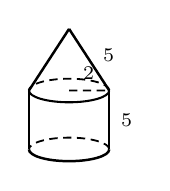
\begin{tikzpicture}[scale=0.68, every node/.style={font=\scriptsize, text=black}]
        \draw[black, line width=0.9pt] (-0.75,-0.95) arc (-180:0:0.75 and 0.22);
        \draw[black, line width=0.65pt, densely dashed] (0.75,-0.95) arc (0:180:0.75 and 0.22);
        \draw[black, line width=0.9pt] (-0.75,-0.95) -- (-0.75,0.15) (0.75,-0.95) -- (0.75,0.15);
        \draw[black, line width=0.75pt] (-0.75,0.15) arc (-180:0:0.75 and 0.22);
        \draw[black, line width=0.65pt, densely dashed] (0.75,0.15) arc (0:180:0.75 and 0.22) (0,0.15) -- (0.75,0.15);
        \draw[black, line width=0.9pt] (0,1.30) -- (-0.75,0.15) (0,1.30) -- (0.75,0.15);
        \node[above=0.5pt] at (0.38,0.15) {$2$};
        \node[right=1pt] at (0.75,-0.40) {$5$};
        \node[right=1pt] at (0.40,0.80) {$5$};
      \end{tikzpicture}
    \end{minipage}
  \end{tcolorbox}
\end{minipage}

\vspace{16pt}
% --- E3 Explain: Formula Summary & Parameter Trap Table ---
\secbar{ផ្នែកទី២ ៖ សង្ខេបរូបមន្តផ្ទៃក្រឡាកោន និងតារាងការពារអន្ទាក់ទិន្នន័យ \enbf{(E3 - Explain)}}{សង្ខេបរួមគ្នា \en{6 min}}

\begin{tcolorbox}[
  enhanced, sharp corners, colback=white, colframe=black,
  boxrule=0.9pt, boxsep=4.5pt, top=9pt, bottom=9pt, left=6pt, right=6pt
]
  {\renewcommand{\arraystretch}{1.95}\footnotesize
  \begin{tabular}{|L{4.85cm}|L{6.15cm}|L{6.10cm}|}
    \hline
    \cellcolor{headgray}\textbf{បរិមាណនៃកោនបរិវត្ត} & \cellcolor{headgray}\textbf{រូបមន្តគណនា} & \cellcolor{headgray}\textbf{អន្ទាក់ទិន្នន័យដែលត្រូវប្រយ័ត្ន!} \\
    \hline
    $1.$ ទំនាក់ទំនង $r$, កម្ពស់ $h$, ជនេត្រ $s$ & $s^2 = h^2 + r^2 \;\Rightarrow\; s = \sqrt{\blank{1.9cm}}$ & បើប្រាប់អង្កត់ផ្ចិត $d$ ត្រូវរក $r = \dfrac{d}{2}$ ជាមុន! \\
    \hline
    $2.$ ផ្ទៃក្រឡាខាងនៃកោន ($S_l$) & $S_l = \pi \times \blank{0.8cm} \times \blank{0.8cm}$ & ប្រើ \textbf{ជនេត្រ $s$} (ហាមយកកម្ពស់កែង $h$ ជំនួស $s$!) \\
    \hline
    $3.$ ផ្ទៃក្រឡាទាំងអស់នៃកោន ($S_T$) & $S_T = S_l + B = \pi r s + \pi r^2 = \pi r(\blank{1.4cm})$ & បូកផ្ទៃថាសបាតតែ \textbf{១} ($B = \pi r^2$) \\
    \hline
  \end{tabular}}\\[9pt]
  $\bullet$ \textbf{ប្រៀបធៀបសូលីតបាតថាស៖}
  \chkbox\ ស៊ីឡាំង៖ $S_l = 2\pi rh,\; S_T = 2\pi rh + 2\pi r^2$ \hspace{0.3cm}
  \chkbox\ កោន៖ $S_l = \pi rs,\; S_T = \pi rs + \pi r^2$\\[7pt]
  $\bullet$ \textbf{ធនាគារហេតុផល៖}
  \cnum{1} $r = \dfrac{d}{2}$ \;\textbar\;
  \cnum{2} ពីតាករ $s = \sqrt{h^2+r^2}$ \;\textbar\;
  \cnum{3} $S_l = \pi r s,\; S_T = \pi r(s+r)$ \;\textbar\;
  \cnum{4} សូលីតផ្សំ/កោនកាត់៖ គិតតែផ្ទៃខាងក្រៅពិត
\end{tcolorbox}

\newpage

% ============================================================================
% ទំព័រទី ២៖ E4 (ប្រតិបត្តិ ក និង ខ ទំ.២២២) + E5 (លំហាត់ចង្កៀងគោមទី៧ & Exit Check) + កិច្ចការផ្ទះ
% ============================================================================

\secbar{ផ្នែកទី៣ ៖ លំហាត់ប្រៀបធៀបអន្ទាក់ទិន្នន័យ \enbf{---} ប្រតិបត្តិ ក និង ខ ទំព័រ ២២២ \enbf{(E4 - Elaborate)}}{អនុវត្ត \en{10 min}}

\noindent
\begin{minipage}[t]{9.4cm}\vspace{0pt}
  \begin{tcolorbox}[
    enhanced, sharp corners, colback=white, colframe=black, equal height group=rowE4,
    boxrule=0.85pt, boxsep=3pt, top=5pt, bottom=5pt, left=5.5pt, right=5.5pt
  ]\raggedright
    \textbf{៣.ក ប្រតិបត្តិ ក (ទំ.២២២, $\pi\approx 3.14$)៖ ប្រយ័ត្ន $d$ និង $h$!}\\
    ពិនិត្យសញ្ញាកែងត្រង់ផ្ចិតបាតនៃកោនខាងក្រោម៖
    \begin{center}
      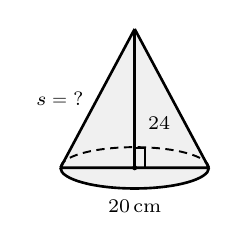
\begin{tikzpicture}[scale=0.82, every node/.style={font=\scriptsize, text=black}]
        \coordinate (V1) at (0,1.40);
        \coordinate (O1) at (0,-0.75);
        \coordinate (L1) at (-1.15,-0.75);
        \coordinate (R1) at (1.15,-0.75);
        \fill[gray!12] (L1) -- (V1) -- (R1) arc (0:-180:1.15 and 0.32);
        \draw[black, line width=0.95pt] (L1) arc (-180:0:1.15 and 0.32) (V1) -- (L1) (V1) -- (R1) (L1) -- (R1);
        \draw[black, line width=0.7pt, densely dashed] (R1) arc (0:180:1.15 and 0.32);
        \draw[black, line width=0.85pt] (V1) -- (O1);
        \rightbox[0.14]{V1}{O1}{R1}
        \fill[black] (O1) circle (1.1pt);
        \node[right=1.5pt] at (0,-0.05) {$24$};
        \node[below=1pt] at (0,-1.05) {$20\unit{cm}$};
        \node[left=1.5pt] at ($0.5*(V1)+0.5*(L1)$) {$s=?$};
      \end{tikzpicture}
    \end{center}
    $1.$ អង្កត់ផ្ចិត $d = 20\unit{cm} \Rightarrow$ កាំបាត $r = \dfrac{20}{2} = \blank{1.2cm}\unit{cm}$\\[4pt]
    $2.$ រកជនេត្រ $s$ (តាមពីតាករ ព្រោះ $h = 24\unit{cm}$)៖\\[3pt]
    \hspace*{0.2cm}$s = \sqrt{24^2 + (\blank{0.8cm})^2} = \sqrt{\blank{1.3cm}} = \blank{1.2cm}\unit{cm}$\\[4pt]
    $3.$ $S_T = \pi r(s+r) \approx 3.14\times\blank{0.8cm}\times(\blank{0.8cm}+\blank{0.8cm}) = \blank{1.5cm}\unit{cm}^2$
  \end{tcolorbox}
\end{minipage}%
\hfill
\begin{minipage}[t]{9.4cm}\vspace{0pt}
  \begin{tcolorbox}[
    enhanced, sharp corners, colback=white, colframe=black, equal height group=rowE4,
    boxrule=0.85pt, boxsep=3pt, top=5pt, bottom=5pt, left=5.5pt, right=5.5pt
  ]\raggedright
    \textbf{៣.ខ ប្រតិបត្តិ ខ (ទំ.២២២, $\pi\approx 3.14$)៖ ស្គាល់ $r$ និង $s$ ស្រាប់!}\\
    ពិនិត្យបន្ទាត់ដាច់ៗពីផ្ចិតទៅគែមថាសបាតខាងក្រោម៖
    \begin{center}
      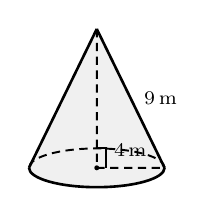
\begin{tikzpicture}[scale=0.82, every node/.style={font=\scriptsize, text=black}]
        \coordinate (V2) at (0,1.40);
        \coordinate (O2) at (0,-0.75);
        \coordinate (L2) at (-1.05,-0.75);
        \coordinate (R2) at (1.05,-0.75);
        \fill[gray!12] (L2) -- (V2) -- (R2) arc (0:-180:1.05 and 0.30);
        \draw[black, line width=0.95pt] (L2) arc (-180:0:1.05 and 0.30) (V2) -- (L2) (V2) -- (R2);
        \draw[black, line width=0.7pt, densely dashed] (R2) arc (0:180:1.05 and 0.30) (V2) -- (O2) -- (R2);
        \rightbox[0.14]{V2}{O2}{R2}
        \fill[black] (O2) circle (1.1pt);
        \node[above=0.5pt] at (0.52,-0.75) {$4\unit{m}$};
        \node[right=1.5pt] at ($0.5*(V2)+0.5*(R2)$) {$9\unit{m}$};
      \end{tikzpicture}
    \end{center}
    $1.$ កាំបាត $r = \blank{1.1cm}\unit{m}$,\; ជនេត្រ $s = \blank{1.1cm}\unit{m}$\\
    \hspace*{0.2cm}\textit{(តើចាំបាច់ប្រើទ្រឹស្ដីបទពីតាករទៀតឬទេ? \chkbox\ ចាំបាច់ \;\chkbox\ មិនចាំបាច់)}\\[4pt]
    $2.$ ផ្ទៃក្រឡាខាង៖ $S_l = 3.14 \times \blank{0.8cm} \times \blank{0.8cm} = \blank{1.4cm}\unit{m}^2$\\[4pt]
    $3.$ ផ្ទៃក្រឡាទាំងអស់៖\\
    \hspace*{0.2cm}$S_T = \pi r(s+r) \approx 3.14\times 4\times(\blank{0.8cm}+\blank{0.8cm}) = \blank{1.5cm}\unit{m}^2$
  \end{tcolorbox}
\end{minipage}

\vspace{11pt}
% --- E5 Evaluate: Lampshade Frustum Ex #7 + Exit Check ---
\secbar{ផ្នែកទី៤ ៖ វាយតម្លៃ \enbf{---} លំហាត់ចង្កៀងគោមទី៧ \enbf{(}ទំ\enbf{.}២២៧\enbf{)} និង \enbf{Exit Check (E5)}}{ធ្វើដោយឯករាជ្យ \en{10 min}}

\noindent
\begin{minipage}[t]{10.3cm}\vspace{0pt}
  \begin{tcolorbox}[
    enhanced, sharp corners, colback=white, colframe=black, equal height group=rowE5,
    boxrule=0.85pt, boxsep=3pt, top=6pt, bottom=6pt, left=5.5pt, right=5.5pt
  ]
    \textbf{៤.ក លំហាត់ទី៧ (ទំ.២២៧, $\pi\approx 3.14$)៖ ចង្កៀងគោម (កោនធំ ដក កោនតូច)}\\[4.5pt]
    \begin{minipage}[c]{6.3cm}\raggedright
      គេផលិតចង្កៀងគោមដោយកាត់កោនតូច ($r_2=7\unit{cm},\; s_2=10.5\unit{cm}$) ចេញពីកោនធំ ($r_1=21\unit{cm},\; s_1=55\unit{cm}$) ដូចរូប៖\\[4.5pt]
      $1.$ ចង្កៀងគោមចំហមាត់លើ-ក្រោម ដូចនេះគណនាតែផ្ទៃក្រឡាខាង៖\\[3.5pt]
      $\bullet$ ផ្ទៃខាងកោនធំ៖\\
      \hspace*{0.15cm}$S_{l1} = 3.14\times 21\times 55 = \blank{1.65cm}\unit{cm}^2$\\[3.5pt]
      $\bullet$ ផ្ទៃខាងកោនតូច៖\\
      \hspace*{0.15cm}$S_{l2} = 3.14\times 7\times 10.5 = \blank{1.65cm}\unit{cm}^2$
    \end{minipage}%
    \hfill
    \begin{minipage}[c]{2.9cm}
      \centering
      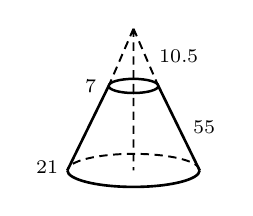
\begin{tikzpicture}[scale=0.75, every node/.style={font=\scriptsize, text=black}]
        \coordinate (Top) at (0,1.55);
        \draw[black, line width=0.7pt, densely dashed] (Top) -- (-0.42,0.58) (Top) -- (0.42,0.58) (0,1.55) -- (0,-0.85);
        \draw[black, line width=0.95pt] (-0.42,0.58) -- (-1.12,-0.85) (0.42,0.58) -- (1.12,-0.85);
        \draw[black, line width=0.9pt] (0,0.58) ellipse (0.42 and 0.12);
        \draw[black, line width=0.95pt] (-1.12,-0.85) arc (-180:0:1.12 and 0.28);
        \draw[black, line width=0.7pt, densely dashed] (1.12,-0.85) arc (0:180:1.12 and 0.28);
        \node[left=1pt] at (-0.42,0.58) {$7$};
        \node[left=1pt] at (-1.05,-0.80) {$21$};
        \node[right=1pt] at (0.80,-0.12) {$55$};
        \node[right=1pt] at (0.22,1.08) {$10.5$};
      \end{tikzpicture}
    \end{minipage}\\[6pt]
    $2.$ ផ្ទៃក្រឡាចង្កៀងគោម៖ $S = S_{l1} - S_{l2} = \blank{1.6cm} - \blank{1.5cm} = \blank{1.8cm}\unit{cm}^2$ ។
  \end{tcolorbox}
\end{minipage}%
\hfill
\begin{minipage}[t]{8.5cm}\vspace{0pt}
  \begin{tcolorbox}[
    enhanced, sharp corners, colback=white, colframe=black, equal height group=rowE5,
    boxrule=0.85pt, boxsep=3pt, top=6pt, bottom=6pt, left=5.5pt, right=5.5pt
  ]\raggedright
    \textbf{៤.ខ សំណួរត្រួតពិនិត្យរហ័ស (\en{Exit Check})៖}\\
    គូសវង់ជុំវិញអក្សរនៃចម្លើយត្រឹមត្រូវតែមួយគត់៖\\[6.5pt]
    \textbf{សំណួរទី១៖} រូបមន្តផ្ទៃក្រឡាទាំងអស់នៃកោនបរិវត្តគឺ៖\\[2.5pt]
    \hspace*{0.10cm}\textbf{ក.} $\pi r h + \pi r^2$ \hspace{0.25cm} \textbf{ខ.} $2\pi r s + \pi r^2$ \hspace{0.25cm} \textbf{គ.} $\pi r(s + r)$\\[7.5pt]
    \textbf{សំណួរទី២៖} កោនបរិវត្តមួយមានកាំបាត $r = 3\unit{cm}$ និងកម្ពស់ $h = 4\unit{cm}$ មានជនេត្រ $s$ ស្មើនឹង៖\\[2.5pt]
    \hspace*{0.15cm}\textbf{ក.} $4\unit{cm}$ \hspace{0.65cm} \textbf{ខ.} $5\unit{cm}$ \hspace{0.65cm} \textbf{គ.} $7\unit{cm}$\\[7.5pt]
    \textbf{សំណួរទី៣៖} សូលីតផ្សំដោយស៊ីឡាំងបិទបាតក្រោមមួយ និងដំបូលកោនបន្តុបពីលើ មានផ្ទៃក្រឡាសរុបស្មើនឹង៖\\[2.5pt]
    \hspace*{0.10cm}\textbf{ក.} $\pi r^2 + 2\pi rh + \pi rs$ \hspace{0.25cm} \textbf{ខ.} $2\pi r^2 + 2\pi rh + \pi rs$
  \end{tcolorbox}
\end{minipage}

\vspace{11pt}
% --- Step 5 Homework Box ---
\secbar{ផ្នែកទី៥ ៖ កិច្ចការផ្ទះ និងបណ្ដាំផ្ញើ \enbf{(}ទំព័រ ២២៧ លំហាត់ទី៦ និងទំព័រ ២២៩ លំហាត់ទី១២\enbf{)}}{ធ្វើនៅផ្ទះក្នុងសៀវភៅសរសេរ}

\begin{tcolorbox}[
  enhanced, sharp corners, colback=panelgray, colframe=black,
  boxrule=0.85pt, boxsep=3.5pt, top=6pt, bottom=6pt, left=6pt, right=6pt
]
  \begin{minipage}[c]{14.2cm}\raggedright
    $1.$ \textbf{លំហាត់ទី៦ (ទំ.២២៧, រូបទី ១ ខាងស្ដាំ)៖} គណនាផ្ទៃក្រឡាខាង ($S_l$) និងផ្ទៃក្រឡាសរុប ($S_T$) នៃកោនដែលមានកាំបាត $r=9\unit{cm}$ និងកម្ពស់ $h=16\unit{cm}$ (រកជនេត្រ $s = \sqrt{16^2+9^2}$ ជាមុន, $\pi\approx 3.14$) ។\\[3pt]
    $2.$ \textbf{លំហាត់ទី១២ (ទំ.២២៩)៖} គណនាផ្ទៃក្រឡាសរុបនៃកោន បើផ្ទៃក្រឡាបាតមានរង្វាស់ $B = 160\unit{cm}^2$ និងជនេត្រមានរង្វាស់ $s = 12\unit{cm}$ (យក $\pi \approx 3.142$) ។\\[3pt]
    $3.$ \textbf{អានមេរៀនបន្ទាប់៖} ១៧.២ ការគណនាមាឌនៃព្រីស (ទំ.២២២\,\en{--}\,២២៣) ។
  \end{minipage}%
  \hfill
  \begin{minipage}[c]{3.8cm}
    \centering
    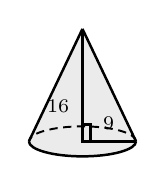
\begin{tikzpicture}[scale=0.68, every node/.style={font=\scriptsize, text=black}]
      \coordinate (V) at (0,1.35);
      \coordinate (O) at (0,-0.75);
      \coordinate (L) at (-1.00,-0.75);
      \coordinate (R) at (1.00,-0.75);
      \fill[gray!16] (L) -- (V) -- (R) arc (0:-180:1.00 and 0.28);
      \draw[black, line width=0.9pt] (L) arc (-180:0:1.00 and 0.28) (V) -- (L) (V) -- (R);
      \draw[black, line width=0.7pt, densely dashed] (R) arc (0:180:1.00 and 0.28);
      \draw[black, line width=0.85pt] (V) -- (O) -- (R);
      \rightbox[0.15]{V}{O}{R}
      \node[left=1pt] at (0,-0.10) {$16$};
      \node[above=0.5pt] at (0.50,-0.75) {$9$};
    \end{tikzpicture}
  \end{minipage}
\end{tcolorbox}

\end{document}
